\documentclass[a4paper]{article} 
\addtolength{\hoffset}{-2.25cm}
\addtolength{\textwidth}{4.5cm}
\addtolength{\voffset}{-3.25cm}
\addtolength{\textheight}{5cm}
\setlength{\parskip}{0pt}
\setlength{\parindent}{0in}

%----------------------------------------------------------------------------------------
%	PACKAGES AND OTHER DOCUMENT CONFIGURATIONS
%----------------------------------------------------------------------------------------

\usepackage{blindtext} % Package to generate dummy text
% \usepackage{charter} % Use the Charter font
\usepackage[utf8]{inputenc} % Use UTF-8 encoding
\usepackage{microtype} % Slightly tweak font spacing for aesthetics
\usepackage[english, ngerman]{babel} % Language hyphenation and typographical rules
\usepackage{amsthm, amsmath, amssymb} % Mathematical typesetting
\usepackage{float} % Improved interface for floating objects
\usepackage[final, colorlinks = true, 
            linkcolor = black, 
            citecolor = black]{hyperref} % For hyperlinks in the PDF
\usepackage{graphicx, multicol} % Enhanced support for graphics
\usepackage{xcolor} % Driver-independent color extensions
\usepackage{marvosym, wasysym} % More symbols
\usepackage{rotating} % Rotation tools
\usepackage{censor} % Facilities for controlling restricted text
\usepackage{listings, style/lstlisting} % Environment for non-formatted code, !uses style file!
\usepackage{pseudocode} % Environment for specifying algorithms in a natural way
\usepackage{style/avm} % Environment for f-structures, !uses style file!
\usepackage{booktabs} % Enhances quality of tables
\usepackage{tikz-qtree} % Easy tree drawing tool
\tikzset{every tree node/.style={align=center,anchor=north},
         level distance=2cm} % Configuration for q-trees
\usepackage{style/btree} % Configuration for b-trees and b+-trees, !uses style file!
\usepackage[backend=biber,style=numeric,
            sorting=nyt]{biblatex} % Complete reimplementation of bibliographic facilities
\addbibresource{ecl.bib}
\usepackage{csquotes} % Context sensitive quotation facilities
\usepackage[ddmmyyyy]{datetime} % Uses YEAR-MONTH-DAY format for dates
%\renewcommand{\dateseparator}{-} % Sets dateseparator to '-'
\usepackage{fancyhdr} % Headers and footers
\pagestyle{fancy} % All pages have headers and footers
\fancyhead{}\renewcommand{\headrulewidth}{0pt} % Blank out the default header
\fancyfoot[L]{} % Custom footer text
\fancyfoot[C]{} % Custom footer text
\fancyfoot[R]{\thepage} % Custom footer text
\newcommand{\note}[1]{\marginpar{\scriptsize \textcolor{red}{#1}}} % Enables comments in red on margin

%----------------------------------------------------------------------------------------

\usepackage{mathtools}
\DeclarePairedDelimiter\ceil{\lceil}{\rceil}
\DeclarePairedDelimiter\floor{\lfloor}{\rfloor}
\begin{document}
	%-------------------------------
	%	TITLE SECTION
	%-------------------------------
	
	\fancyhead[C]{}
	\hrule \medskip % Upper rule
	\begin{minipage}{0.295\textwidth} 
		\raggedright
		\footnotesize
		Université de Lorraine\hfill\\   
		Télécom Nancy - 1A\hfill\\
		Omar CHIDA
	\end{minipage}
	\begin{minipage}{0.4\textwidth} 
		\centering 
		\large 
		Travaux Dirigés 3\\ 
		\normalsize 
		Langage C\\ 
	\end{minipage}
	\begin{minipage}{0.295\textwidth} 
		\raggedleft
		\today\hfill\\
	\end{minipage}
	\medskip\hrule 
	\bigskip
	
	%-------------------------------
	%	CONTENTS
	%-------------------------------	
	\section*{L'objectif}
	Le but de ce TD est de se familiariser avec :
	\begin{itemize}
		\item l'allocation dynamique de mémoire et l'arithmétique des pointeurs.
		\item lecture des fichiers.
	\end{itemize}

	Dans ce TD, vous devez écrire des fonctions qui charge une image à partir d'un fichier BMP\footnote{Bitmap image file}. Ecrire des fonctions qui effectuent quelques technique de traitement d'image (transformé une image en échelle de gris, effectuer des produits de convolution afin d'appliquer des filtres, ...). \\
	
	\centerline{\Large{Lisez l'intégralité du document avant d'écrire le code.}}
	
	\section*{Généralités, pixels et couleurs}
	Les couleurs sont une sorte de données, mais comment peuvent-elles être représentées dans les ordinateurs? Il y a tant de façons de représenter la couleur, la plus célèbre est la représentation RGBA (RGBA signifie Red, Green, Bleu et Alpha). La plupart des couleurs peuvent être représentées en utilisant un mélange des 3 couleurs fondamentales (le rouge, vert et bleu). L'absence de ces 3 couleurs signifie le noir et leur présence tous ensemble représente la couleur blanche. L'alpha représente la transparence et ce n'est pas très pertinent dans ce que nous allons faire. Généralement, 8 bits sont plus que suffisants pour stocker chacune de ces 3 couleurs et la transparence. Ainsi, chaque canal de couleur est représenté par 1 octet en mémoire (1 octet pour le rouge, le vert, le bleu et l'alpha) ce qui fait heureusement jusqu'à 4 octets. L'ordre des octets rouge, vert, bleu et alpha varie en fonction du format. Les formats les plus courants sont RGBA et BGRA. Dans le premier format, le rouge est stocké en premier, suivi du vert, du bleu et de l'alpha. Dans le second, le bleu est stocké en premier, suivi du vert, du rouge et de l'alpha. \\
	Il existe deux types d'images, les images vectorielles et les images matricielles. Dans ce dernier, (qui est celui que nous allons traiter) les informations de couleur sont stockées par pixel\footnote{abréviation de picture elements} qui sont les plus petits éléments adressables dans ce type d'images. Une image contient donc $largeur * hauteur$ pixels. \\
	Pour la sutie du TD, si on a une matrice M  de pixels de taille H par L, ou H l'hauteur et L la largeur de l'image alors \texttt{pixels[y][x]} nous donne le pixel à la ligne \texttt{y} et la colonne \texttt{x}.
	
	\section*{Le format de fichier BMP}
	Le format BMP est un format de fichier d'image graphique de type raster\footnote{Cela signifie qu'il stocke des pixels contrairement aux images vectorielles}, utilisé pour stocker des images numériques. Le format BMP est connu pour sa simplicité car aucune compression n'est effectuée\footnote{en fait, certaines techniques de compression peuvent être utilisées mais ce n'est pas très courant}. \\
	Un fichier BMP contient au moins 3 sections :
	
	\subsubsection*{Bitmap File Header}
	Cette entête, qui a une taille globale de 14 octets, existe au début de chaque fichier BMP. Elle contient des métadonnées sur le fichier en général. Les champs de cette entête sont dans l'ordre :
	\begin{itemize}
		\item \textbf{Signature :} Utilisé pour vérifier que le format de fichier est BMP. Il occupe deux octets en mémoire. le premier octet doit être égal au caractère ascii \texttt{B} et le second doit être égal au caractère ascii \texttt{M}.
		\item \textbf{File size : } Occupe 4 octets. Il est utilisé pour indiquer la taille du fichier en octets.
		\item \textbf{Reserved : } Cela occupe au total 4 octets et est réservé à l'application qui crée l'image. Cela ne sera pas très intéressant pour nous.
		\item \textbf{Offset to pixels : } C'est un champ très important, qui indique combien d'octets nous devons sauter à partir du début du fichier pour trouver le tableau de pixels qui contient des informations sur la couleur de chaque pixel (plus à ce sujet plus tard)
	\end{itemize}
	
	\subsubsection*{DIB Header}
		Cet en-tête se trouve juste après le \textit{Bitmap File Header}. Cette section est importante car elle stocke des informations détaillées sur l'image bitmap et définit le format de pixel. Parmi les nombreux champs que cet en-tête définit, nous ne serons intéressés que par quelques-uns d'entre eux: taille de l'en-tête, largeur, hauteur, nombre de plans de couleur, les bits par pixel et masque de bits du rouge, bleu, vert et alpha.
		Les premiers champs que cet en-tête contient sont dans l'ordre :
		\begin{center}
			\begin{tabular}{ | p{4cm} | p{0.8cm} | p{1.2cm} | p{10cm} | } 
				\hline
				\textbf{Champ}  				& \textbf{Taille}& \textbf{Type} & \textbf{Description} \\ 
				\hline
				\texttt{Header Size}  		    & 4o 	 & int  & la taille de cet section \\ 
				\hline
				\texttt{Image Width} 			& 4o 	 & int  & la largeur du bitmap en pixels (de l'image) \\ 
				\hline
				\texttt{Image Height} 		    & 4o     & int  & la hauteur du bitmap en pixels (de l'image) \\
				\hline
				\texttt{Planes} 				& 2o 	 & unsigned short& le nombre de plans de couleur (doit être 1) \\
				\hline
				\texttt{Bits per pixel (BPP)}   & 2o     & unsigned short& le nombre de bits par pixel, qui est la profondeur de couleur de l'image. Les valeurs typiques sont 1, 4, 8, 16, 24 et 32. \\
				\hline
				\texttt{Compression} 			& 4o     & int  & la méthode de compression utilisée (Pas important dans notre cas). \\
				\hline
				\texttt{X pixels per meter} 	& 4o     & int  & la résolution horizontale de l'image (pixel par mètre). (Pas important dans notre cas) \\
				\hline
				\texttt{Y pixels per meter} 	& 4o     & int  & la résolution verticale de l'image (pixel par mètre). (Pas important dans notre cas) \\
				\hline
				\texttt{Colors in color table}  & 4o     & int  & le nombre de couleurs dans la palette de couleurs. (Pas important dans notre cas) \\
				\hline
				\texttt{Important color count}  & 4o     & int  & le nombre de couleurs importantes utilisées (généralement ignoré). \\
				\hline
				\texttt{Red channel bitmask} 	& 4o     & unsigned int  & Masque binaire de canal rouge. En utilisant un \texttt{ET} binaire avec les données de pixel ca va donner la valeur de couleur rouge du pixel \\
				\hline
				\texttt{Green channel bitmask}   & 4o 	 & unsigned int  & Masque binaire de canal vert. En utilisant un \texttt{ET} binaire avec les données de pixel ca va donner la valeur de couleur vert du pixel \\
				\hline
				\texttt{Blue channel bitmask}   & 4o 	 & unsigned int  & Masque binaire de canal bleu. En utilisant un \texttt{ET} binaire avec les données de pixel ca va donner la valeur de couleur bleu du pixel \\
				\hline
				\texttt{Alpha channel bitmask}  & 4o     & unsigned int  & Masque binaire de canal alpha, En utilisant un \texttt{ET} binaire avec les données de pixel ca va donner la valeur de l'alpha du pixel \\
				\hline
			\end{tabular}
		\end{center}	
		Les champs restants dans l'en-tête DIB ne sont pas pertinents dans notre cas, donc on va les ignorers.
	
	\subsubsection*{Pixel Array}
	Il s'agit d'un tableau contenant les données de chaque pixel de l'image. Les données de pixels sont stockées telles qu'elles apparaissent dans l'image en allant de gauche à droite et de haut en bas. Ce qui signifie que le premier pixel du tableau correspond au pixel en haut à gauche de l'image.\\
	Chaque ligne du tableau de pixels est complétée à un multiple de 4 octets de taille. Heureusement pour nous, nous ne traiterons que des données de pixels de 4 octets, donc nous n'avons de toute façon pas à gérer ce padding.\\
	
	Voici un tableau qui représente la façon dont le tableau de pixels est stocké dans le fichier bmp. \texttt{h} représente la hauteur et \texttt{w} représente la largeur de l'image.
	\begin{center}
		\begin{tabular}{ | p{2.2cm} | p{2.2cm} | p{2.2cm} | p{1.5cm} | p{2.2cm} | p{1.5cm} | }
			\hline
			\multicolumn{6}{|c|}{Données d'image} \\
			\multicolumn{6}{|c|}{Tableau de pixels [y][x]} \\
			\hline
			pixel[h-1][0] & pixel[h-1][1] & pixel[h-1][2] & ... & pixel[h-1][w-1] & Padding \\
			\hline
			pixel[h-2][0] & pixel[h-2][1] & pixel[h-2][2] & ... & pixel[h-2][w-1] & Padding \\
			\hline
			pixel[h-3][0] & pixel[h-3][1] & pixel[h-3][2] & ... & pixel[h-3][w-3] & Padding \\
			\hline
			\multicolumn{6}{|c|}{...} \\
			\multicolumn{6}{|c|}{...} \\
			\multicolumn{6}{|c|}{...} \\
			\hline
			pixel[2][0] & pixel[2][1] & pixel[2][2] & ... & pixel[2][w-1] & Padding \\
			\hline
			pixel[1][0] & pixel[1][1] & pixel[1][2] & ... & pixel[1][w-1] & Padding \\
			\hline
			pixel[0][0] & pixel[0][1] & pixel[0][2] & ... & pixel[0][w-3] & Padding \\
			\hline
		\end{tabular}
		% \caption{Le tableau de pixels indexé par y, x}
	\end{center}
	
	\section*{Produit de convolution sur les images}
	L'image est une forme d'un signal discret bidimensionnel. Par conséquent, les filtres peuvent être appliqués en utilisant des produits de convolution. Faire des produits de convolution sur des images est assez simple. Vous prenez un noyau (également appelé matrice de convolution) et le faites glisser à travers l'image en multipliant chaque cellule de la matrice par le pixel correspondant, puis il suffit d'additionner tous les valeurs obtenus. Et enfin mettre le pixel au centre de la matrice de convolution à la somme que nous avons obtenue.\\ Si cette explication vous semble horrible, je vous recommande de consulter cet \href{https://setosa.io/ev/image-kernels/}{article}. Ce n'est pas si long et ca vous offre une manière interactive de visualiser les produits de convolution sur les images.
	
	\section*{Travail demandé : }
	Le travail requis est divisé en parties. A la fin de chaque partie vous pourrez vérifier votre travail en exécutant les tests. 
	Clonez ce repistory \href{https://github.com/Darhal/TeachingC/tree/main/assignements/pbs3}{Github} avant de passer aux questions. \\
	
	\subsubsection*{Partie 1 : Quelques fonctions utilitaires : Mémoire dynamique, matrices}
	Dans cette partie, vous devrez implémenter quelques fonctions utilitaires afin de passer à la partie suivante. \\
	
	1- Dans le fichier \texttt{matrix.c} implémentez une fonction \texttt{mat\_init(unsigned N, unsigned M, unsigned unit\_size)} qui alloue de la mémoire pour une matrice N par M d'un élément de taille \texttt{unit\_size} octets. Implémenter la fonction \texttt{mat\_free(void** mat)} qui libère la mémoire allouée à la matrice. Si vous êtes bloqué, vous pouvez utiliser le dossier nommé matrix qui contient \texttt{matrix.h} et \texttt{matrix.c} les copier dans votre répertoire source principal.
	\begin{lstlisting}[language=C]
/**
* Allocates memory for N by M matrix that contain elements of unit_size bytes
*/ 
void** mat_init(unsigned N, unsigned M, unsigned unit_size);

/**
* Frees the memory allocated by mat_init
*/
void mat_free(void** mat);
	\end{lstlisting}
	
	\textbf{Toutes les fonctions qui suit dans cette PARTIE doivent être définies avec le mot-clé \texttt{static} et elles doivent être définies en haut du fichier \texttt{image.c} juste après les includes.} \\
	2- Implémentez une fonction appelée \texttt{clz(bits)}\footnote{count leading zeros} qui prend un entier positif comme argument et compte le nombre de bits mis à zéro en allant de gauche à droite jusqu'à ce qu'il atteigne un 1 ou la fin. (Il compte le nombre de zéros avant la première occurrence d'un) \\
	Exemples:
	\begin{lstlisting}[language=C]
Pour 00000000 00000000 00000000 00010000 clz doit retourner : 27
Pour 00000001 00000000 00000000 00010000 clz doit retourner : 7
Pour 00000000 00001000 11111111 00010000 clz doit retourner : 12
Pour 00000000 00000001 11111111 00010000 clz doit retourner : 15
	\end{lstlisting}
 	C'est une question du premier TD. Si vous avez implémenteé cette fonction avec succès, vous pouvez passer à la question suivante. Si vous ne l'avez pas implémenté, c'est probablement le moment de le faire. Si vous êtes bloqué, pas de soucis, vous pouvez toujours passer à la question suivante juste avant cela, vous devez décommenter cette ligne \texttt{\#include "clz/clz.h"} dans \texttt{image.c} comme indiqué dans les commentaires afin que vous puissiez utiliser l'implémentation que j'ai fourni ;). \\
	
	3- Toujours en haut du fichier \texttt{image.c} après les includes, écrivez une fonction statique qui, étant donné un nombre impair \texttt{N}, il recherche les coordonnées des cellules voisines de la cellule centrale dans la matrice NxN.
	\textbf{Exemples :}
	Pour N = 3, la fonction doit retourner le tableau : \texttt{ \{ (-1,-1) (-1,0) (-1,1) (0,-1) (0,0) (0,1) (1,-1) (1,0) (1,1)\} } \\
	En effet : 
	\begin{center}
		\begin{tabular}{ | c | c | c | } 
			\hline
			(-1, -1) & (-1, 0) & (-1, 1) \\
			\hline
			(0, -1) & (0, 0) & (0, 1) \\
			\hline
			(1, -1) & (1, 0) & (1, 1) \\
			\hline
		\end{tabular}
	\end{center}
	
	Pour N = 5, la fonction doit retourner le tableau : \texttt{ \{ (-2,-2) (-2,-1) (-2,0) (-2,1) (-2,2) (-1,-2) (-1,-1) (-1,0) (-1,1) (-1,2) (0,-2) (0,-1) (0,0) (0,1) (0,2) (1,-2) (1,-1) (1,0) (1,1) (1,2) (2,-2) (2,-1) (2,0) (2,1) (2,2)\} } \\
	En effet : 
	\begin{center}
		\begin{tabular}{ | c | c | c | c | c | } 
		\hline
		(-2, -2) & (-2, -1) & (-2, 0) & (-2, 1) & (-2, 2) \\
		\hline
		(-1, -2) & (-1, -1) & (-1, 0) & (-1, 1) & (-1, 2) \\
		\hline
		(0, -2) & (0, -1) & (0, 0) & (0, 1) & (0, 2) \\
		\hline
		(1, -2) & (1, -1) & (1, 0) & (1, 1) & (1, 2) \\
		\hline
		(2, -2) & (2, -1) & (2, 0) & (2, 1) & (2, 2) \\
		\hline
		\end{tabular}
	\end{center}
	La fonction doit avoir le profil suivant : 
	\begin{lstlisting}[language=C]
/**
* Given an impair kernel_size calc_nehgbours will return the (y, x) coordinates relative
* to the central cell. This function returns the coordinates in a linear array where
* the first element is the coordiante of the top left cell going from left to right and from
* top to bottom
*/ 
static vec2* calc_neighbours(unsigned kernel_size)
	\end{lstlisting}
	Si vous êtes bloqué, vous pouvez décommenter l'include du fichier \texttt{neighbours/neighbours.h} afin de pouvoir utiliser la fonction plus tard.\\
	
	4- Il est temps de consolider et de tester votre travail. Compilez ce que vous avez fait et exécutez les tests en utilisant respectivement les commandes \texttt{make} et \texttt{make run}. Si vous avez réussi le premier ensemble de tests (\texttt{Test Set 1}), félicitations, vous pouvez passer à la partie suivante.
	\subsubsection*{Partie 2 : Lecture des fichiers}
	Dans le fichier \texttt{bmp\_loader.c}, vous devrez implémenter les fonctions suivantes. \\
	
	1- Implémentez la fonction \texttt{bmp\_load(bmp* bmp, const char* filename)} qui prend un pointeur vers une structure bmp et un nom de fichier. La fonction doit ouvrir le fichier appelé \texttt{filename}, puis appelle \texttt{bmp\_load\_header}, vérifier qu'il s'agit d'un fichier BMP en vérifiant la signature, puis elle appelle \texttt{bmp\_load\_dib\_header } et \texttt{bmp\_load\_pixels} avant de fermer le fichier à la fin.
	\begin{lstlisting}[language=C]
/**
* Takes a pointer to a bmp struct and a filename
* It opens the file calls bmp_load_header which 
* loads in the header, then verify that its a BMP 
* file, it asserts if its not. otherwise it proceeds
* to call bmp_load_dib_header and then bmp_load_pixels.
* Then it finally closes the file
*/
void bmp_load(bmp* bmp, const char* filename);
	\end{lstlisting}
	2- Implémentez la fonction \texttt{bmp\_load\_header(bmp\_header* header, FILE* file)} qui remplit la structure \texttt{bmp\_header} avec les données correspondantes du fichier \texttt{file}.
	\begin{lstlisting}[language=C]
/**
* Takes a pointer to the bmp_header and a FILE pointer
* It read relevant data from the file and fills the relevant
* bmp_header fields with the necessary data
*/
void bmp_load_header(bmp_header* header,  FILE* file);
	\end{lstlisting}
	3- Implémentez la fonction \texttt{bmp\_load\_dib\_header(bmp\_dib\_header* dib\_header, FILE* file)} qui remplit la structure \texttt{bmp\_dib\_header} avec les données correspondantes du fichier \texttt{file}.
	\begin{lstlisting}[language=C]
/**
* Takes a pointer to the bmp_dib_header and a FILE pointer
* It read relevant data from the file and fills the relevant
* bmp_dib_header fields with the necessary data
*/
void bmp_load_dib_header(bmp_dib_header* dib_header, FILE* file);
	\end{lstlisting}
	4- Implémentez la fonction \texttt{bmp\_load\_pixels(const bmp\_dib\_header* const dib, unsigned** pixels, FILE* file)} qui charge toutes les données de pixels du fichier \texttt{file} dans la matrice \texttt{pixels}.
	\begin{lstlisting}[language=C]
/**
* Takes a pointer to the bmp_dib_header, a pixels matrix and a FILE pointer
* It read the pixel data from the file and then it fills the pixels matrix
*/
void bmp_load_pixels(const bmp_dib_header* const dib, unsigned** pixels, FILE* file);
	\end{lstlisting}
	
	5- Libère la mémoire utilisée dans le struct \texttt{bmp}
	\begin{lstlisting}[language=C]
/**
* Liberates the memory used in the bmp object
*/ 
void bmp_destroy(bmp* bmp);
	\end{lstlisting}

	6- Il est temps de consolider et de tester votre travail. Compilez ce que vous avez fait et exécutez les tests en utilisant respectivement les commandes \texttt{make} et \texttt{make run}. Si vous avez réussi la deuxième ensemble de tests (\texttt{Test Set 2}), félicitations, vous pouvez passer à la partie suivante.
	
	\subsubsection*{Partie 3 : Traitement d'image, convolution}
	Cette dernière partie du TD nous mettra en œuvre une fonction liée à l'image facilitant son traitement.
	
	1- Implémentez la fonction \texttt{init\_image(unsigned width, unsigned height)} qui initalise l'objet image et alloue la matrice des pixels.
	\begin{lstlisting}[language=C]
/**
* Initialize an image by setting width and height
* and allocating the colors matrix
*/
image init_image(unsigned width, unsigned height);
	\end{lstlisting}

	2- La fonction \texttt{convert\_to\_image(const bmp* const bmp)} convert la \texttt{struct bmp} en \texttt{struct image}. La séparation des canaux de couleur doit se produire dans cette fonction (Aide: utilisez la fonction \texttt{clz} et les masques de bits RGB qui existent dans l'en-tête dib)
	\begin{lstlisting}[language=C]
/**
* Takes a bmp const pointer and converts it to an image object
* In order to do this the width, height and the pixels matrix 
* must be copied over to the image struct
*/ 
image convert_to_image(const bmp* const bmp);
	\end{lstlisting}
	
	3- Cette fonction doit copier l'image passée en argument et renvoyer la copie
\begin{lstlisting}[language=C]
/**
* Copy an existing image to another one
*/ 
image copy_image(const image* const img);
\end{lstlisting}

	4- Convertir une image normale en une image en niveaux de gris cela se fait en prenant la moyenne ds composants \texttt{r}, \texttt{g}, \texttt{r}.
	\begin{lstlisting}[language=C]
/**
* Converts an image to grayscale this can be done by averaging
* the R, G and B component of each pixel
*/
void grayscale_image(image* img);
	\end{lstlisting}

	5- Effectue le produit de convolution entre le \texttt{kernel} (qui est une matrice de dimensions \texttt{kernel\_size}) et l'image \texttt{src}, et stocke le resultat dans l'image \texttt{dst}.
	\begin{lstlisting}[language=C]
/**
* Applies a convolution product between the source image and the kernel
* It stores the result in the destination image 
*/
void apply_filter(image* dst, image* src, unsigned kernel_size, float* kernel);
	\end{lstlisting}

	6- Enregistre l'image passée en argument sur le disque. Il crée un fichier appelé nom et stocke les pixels de couleur dans un format BGRA (ce qui signifie que le composant \texttt{B} est écrit en premier, puis \texttt{G} puis \texttt{R} et enfin \texttt{A}).
	\begin{lstlisting}[language=C]
/**
* Converts an image to grayscale this can be done by averaging
* the R, G and B component of each pixel
*/
void save_raw(const image* const img, const char* name);
	\end{lstlisting}
	
	7- Libère la mémoire utilisée par l'image
	\begin{lstlisting}[language=C]
/**
* Liberates the memory related to the image object
*/ 
void destroy_image(image* img);
	\end{lstlisting}
	6- Compilez ce que vous avez fait et exécutez les tests en utilisant respectivement les commandes \texttt{make} et \texttt{make run}. Si vous avez réussi la troisième ensemble de tests (\texttt{Test Set 3}), félicitations, vous pouvez passer à la partie suivante.
	
	\subsubsection*{Partie 4 : Celebrate}
	1- Il est temps de célébrer et de voir ce que vous avez fait exactement. Visitez ce \href{https://rawpixels.net/}{site Web} et téléchargez l'image que vous avez générée précédemment. Afin de voir les résultats, assurez-vous d'avoir les bonnes configurations.
	\begin{figure}[!h]
		\centering
		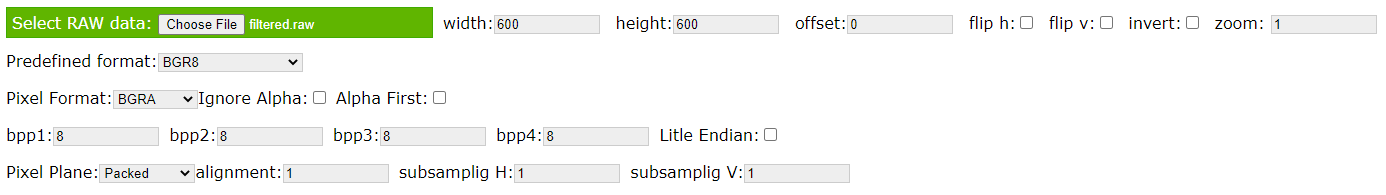
\includegraphics[width=170mm]{resources/raw_pixel_config}
		\caption{Les configurations que vous devez utiliser}
	\end{figure}\\
	2- Essayez d'écrire un programme qui applique un autre filtre (il suffit de changer le noyau) sur la même image et observez le résultat. 
	Pour trouver des noyaux intéressants, visitez cette page \href{https://en.wikipedia.org/wiki/Kernel_(image_processing)}{wikipedia}.\\
	3- Si vous avez encore de l'énergie, implémentez une fonction qui enregistre la structure \texttt{image} sous forme de fichier \texttt{bmp}. De cette façon, vous pouvez visualiser le résultat directement sur votre ordinateur.
	
	\section*{Aide avec les fichiers}
	\begin{lstlisting}[language=C]
// FILE* fopen (const char* filename, const char* mode);
// Opens a file with the name filename, the mode specify the file access mode. It can be:
// "r": read, used for reading existing files
// "w": write, create an empty file to write to. If the file exists then its content is overwritten
// "a": append, opens a file then it writes data at the end of it. The file is created if it does not exist
// Appending b to the mode will open the file as a binary file. 
// NOTE: in our case here we will be using binary files, processing text files isn't that different.

// fseek(FILE* file, long int offset, int origin);
// Sets the position indicator associated with the file to a new position.
// origin can be:
// 		- SEEK_SET : Beginning of file
// 		- SEEK_CUR : Current position of the file pointer
//	    - SEEK_END : End of file
// Offset :
// 		- Binary files: Number of bytes to offset from origin.
// 		- Text files: Either zero, or a value returned by ftell.

// size_t fread (void * ptr, size_t size, size_t count, FILE* file);
// Pointer to a block of memory with at least size*count bytes
// size : size of each elemnt to be read
// count : number of elements to be read, each must be with size of size bytes

// size_t fwrite (const void* ptr, size_t size, size_t count, FILE* stream);
// ptr : pointer to the elments to be written
// size : size in bytes of each elemnt to be written
// count : number of elements each one with size of size bytes
	\end{lstlisting}
\end{document}